\documentclass{article}

\usepackage{graphicx}
\usepackage{tikz}
\usepackage{tikzsymbols}
\usetikzlibrary{calc,patterns,shapes.geometric}
\pagestyle{empty}
\usepackage[margin=0pt]{geometry}
\geometry{papersize={14in,12in}}

\def\centerarc[#1](#2)(#3:#4:#5){\draw[#1] ($(#2)+({#5*cos(#3)},{#5*sin(#3)})$) arc (#3:#4:#5);}

\begin{document}
	\begin{figure}
		\centering
		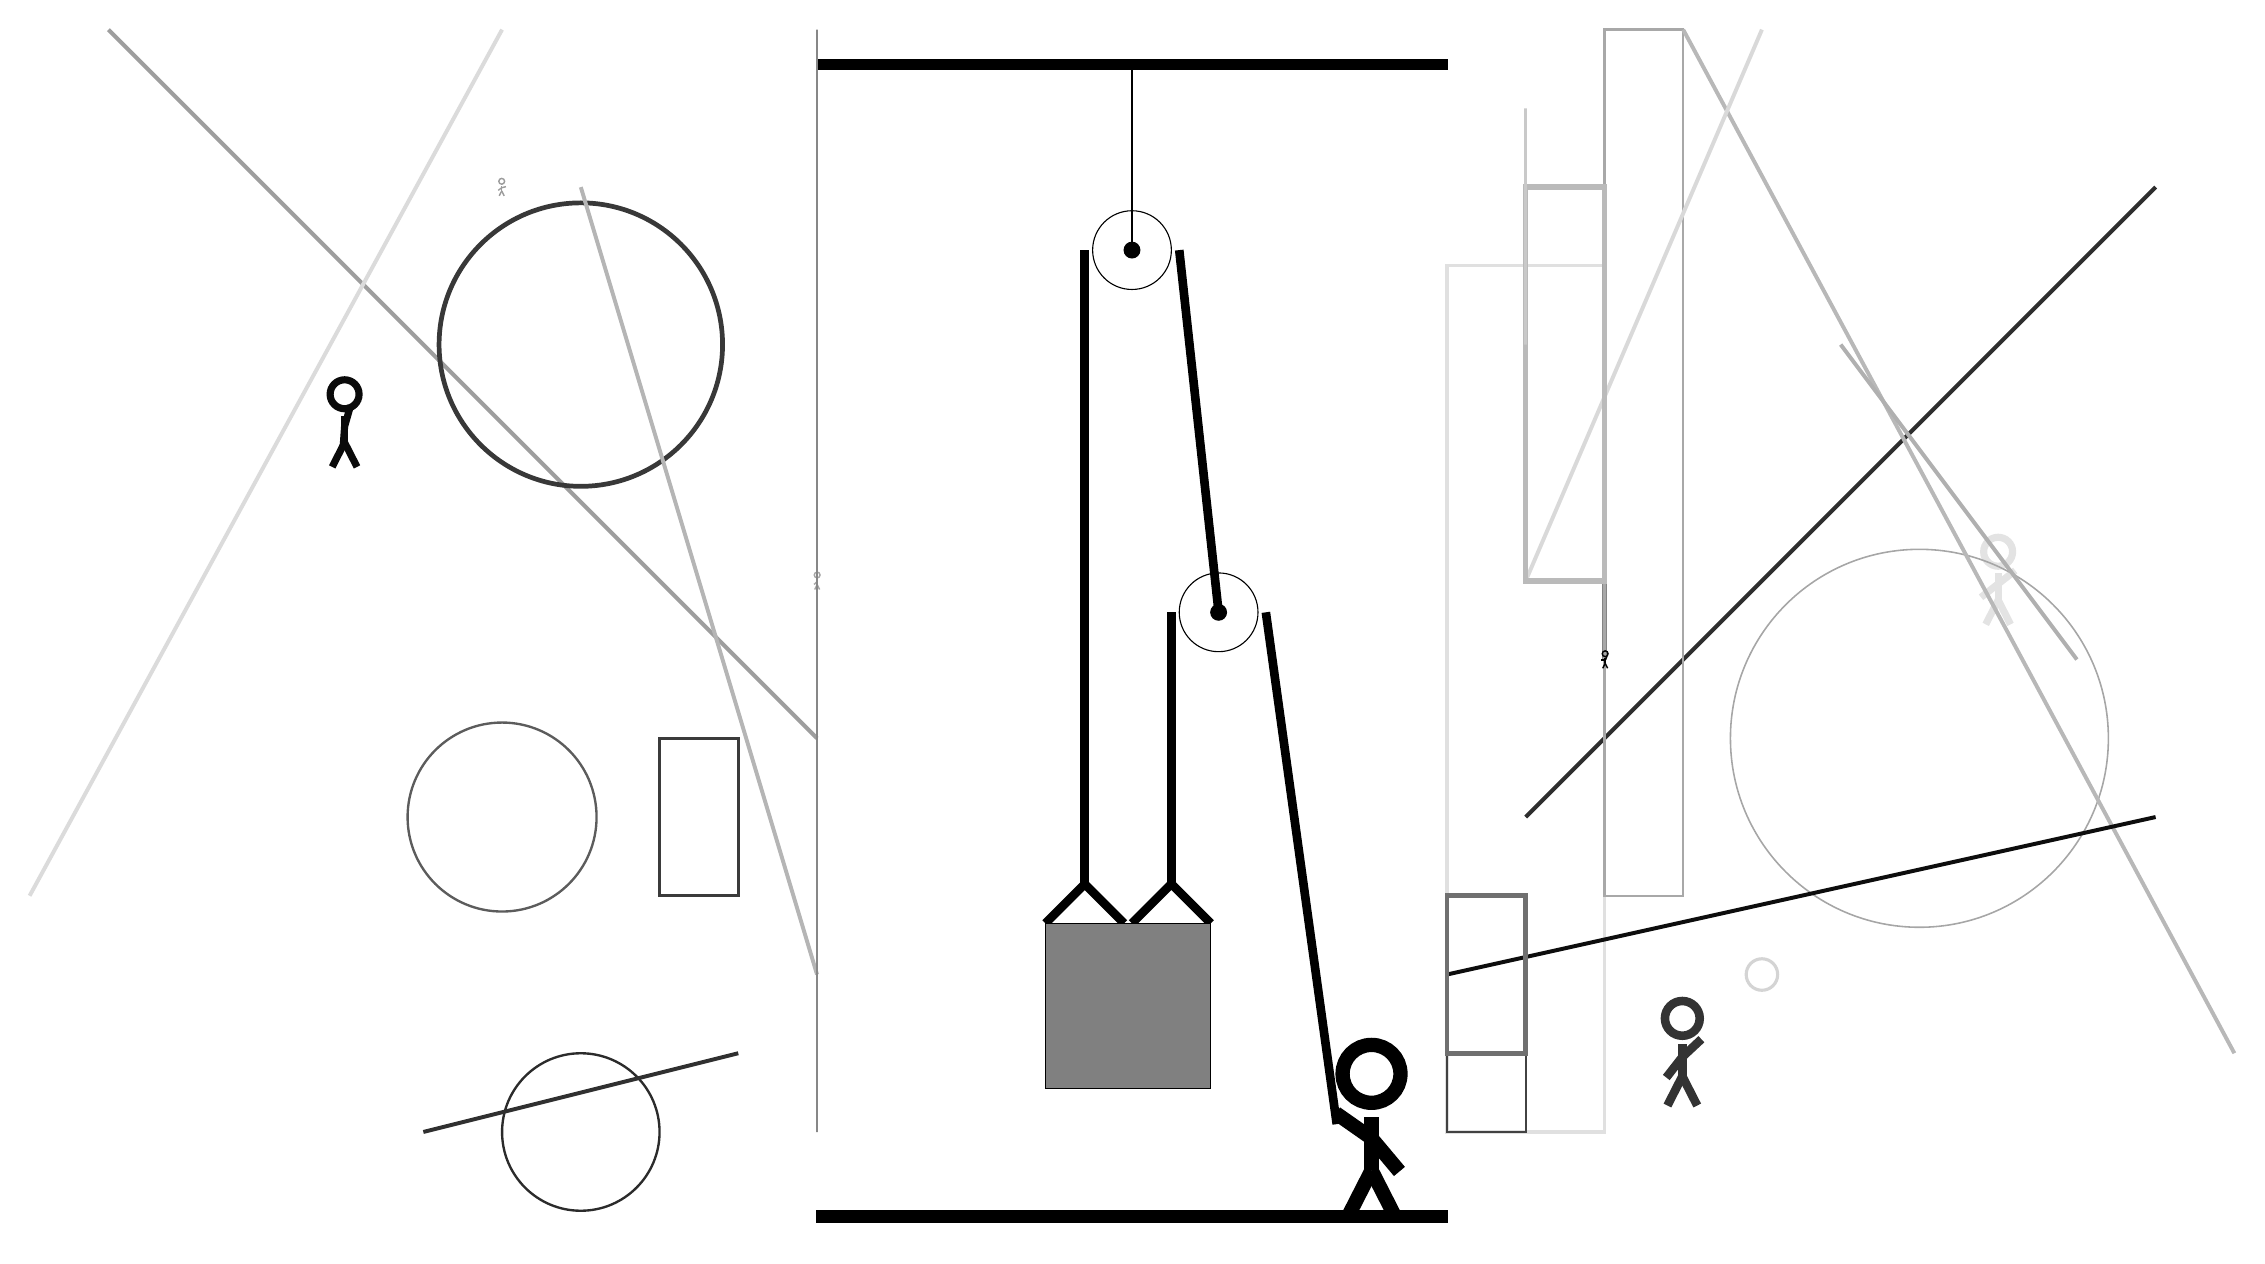
\begin{tikzpicture}
			%%%%% START %%%%%
			
			\draw[fill=black] (-2, 11.5) rectangle (6, 11.625);
			
			\draw (2, 9.2) circle (0.5);
			\draw[fill=black] (2, 9.2) circle (0.1);
			\draw[thick] (2, 9.2) -- (2, 11.5);
			
			\draw (3.1, 4.6) circle (0.5);
			\draw[fill=black] (3.1, 4.6) circle (0.1);
			
			\draw[line width = 1.1mm]  (0.9, 0.65) -- (1.4, 1.15) -- (1.9, 0.65);
			\draw[line width = 1.1mm]  (2.0, 0.65) -- (2.5, 1.15) -- (3.0, 0.65);
			\draw[fill=black!50] (0.9, 0.65) rectangle (3.0, -1.45);
			
			\draw[line width = 1.1mm] (1.4, 9.2) -- (1.4, 1.15);
			\centerarc[line width = 1.1mm](2, 9.2)(0:180:0.6);
			\draw[line width = 1.1mm] (2.6, 9.2) -- (3.1, 4.6);
			\draw[line width = 1.1mm] (2.5, 4.6) -- (2.5, 1.15);
			\centerarc[line width = 1.1mm](3.1, 4.6)(0:180:0.6);
			\draw[line width = 1.1mm] (3.7, 4.6) -- (4.6, -1.9);
			
			\node at (5, -2) {\Strichmaxerl[10][-35][-50]};
			
			\node[line width=0.7mm, color=black!11] at (13, 5) {\Strichmaxerl[5][38][38]};
			
			\draw[line width=0.5mm, color=black!38](-2, 3) -- (-11, 12);
			\draw[line width=0.4mm, color=black!12] (6, 9) rectangle (8, -2);
			\draw[line width=0.5mm, color=black!82](7, 2) -- (15, 10);
			\node[line width=0.6mm, color=black!39] at (-6, 10) {\Strichmaxerl[1][37][14]};
			\draw[line width=0.5mm, color=black!14](-6, 12) -- (-12, 1);
			\draw[line width=0.6mm, color=black!48] (8, 5) rectangle (8, 4);
			
			\draw [line width=0.4mm, color=black!17](10, 0) circle (0.2);
			\draw [line width=0.3mm, color=black!83](-5, -2) circle (1.0);
			\draw[line width=0.5mm, color=black!81](-3, -1) -- (-7, -2);
			
			\node[line width=0.3mm, color=black!96] at (-8, 7) {\Strichmaxerl[5][86][74]};
			
			\draw[line width=0.3mm, color=black!34] (8, 12) rectangle (9, 1);
			\draw [line width=0.3mm, color=black!64](-6, 2) circle (1.2);
			\draw [line width=0.2mm, color=black!35](12, 3) circle (2.4);
			\draw[line width=0.5mm, color=black!28](9, 12) -- (16, -1);
			\draw[line width=0.5mm, color=black!15](7, 5) -- (10, 12);
			\draw[line width=0.4mm, color=black!77] (-3, 3) rectangle (-4, 1);
			
			\node[line width=0.3mm, color=black!35] at (-2, 5) {\Strichmaxerl[1][44][89]};
			\draw[line width=0.7mm, color=black!27] (8, 10) rectangle (7, 5);
			\draw [line width=0.6mm, color=black!78](-5, 8) circle (1.8);
			\draw[line width=0.5mm, color=black!29](-2, 0) -- (-5, 10);
			\draw[line width=0.5mm, color=black!95](6, 0) -- (15, 2);
			\draw[line width=0.3mm, color=black!47] (-2, 12) rectangle (-2, -2);
			\node[line width=0.3mm, color=black!80] at (9, -1) {\Strichmaxerl[6][52][43]};
			\draw[line width=0.3mm, color=black!74] (7, -1) rectangle (6, -2);
			
			\draw[line width=0.4mm, color=black!21] (7, 11) rectangle (7, 8);
			\draw[line width=0.5mm, color=black!31](11, 8) -- (14, 4);
			\draw[line width=0.6mm, color=black!56] (6, 1) rectangle (7, -1);
			\node[line width=0.5mm, color=black!99] at (8, 4) {\Strichmaxerl[1][0][66]};
			
			
			\draw[fill=black] (-2, -3) rectangle (6, -3.15);
			
			%%%%% END %%%%%
		\end{tikzpicture}
	\end{figure}	
\end{document}